\subsection{Elevation Scan}
We performed an elevation scan from the horizon \SI{10}{\degree} to the zenith \SI{90}{\degree} at different  azimuth angles. We chose an angular step size of \SI{1}{\degree}. This step size was chosen as a compromise between measurement time and angular resolution. For these Measurements we made sure that the sun does not cross the scan path. We performed two measurements at different times during the day.

\begin{figure}[ht]
\centering
\begin{subfigure}[t]{0.45\textwidth}
    \centering
    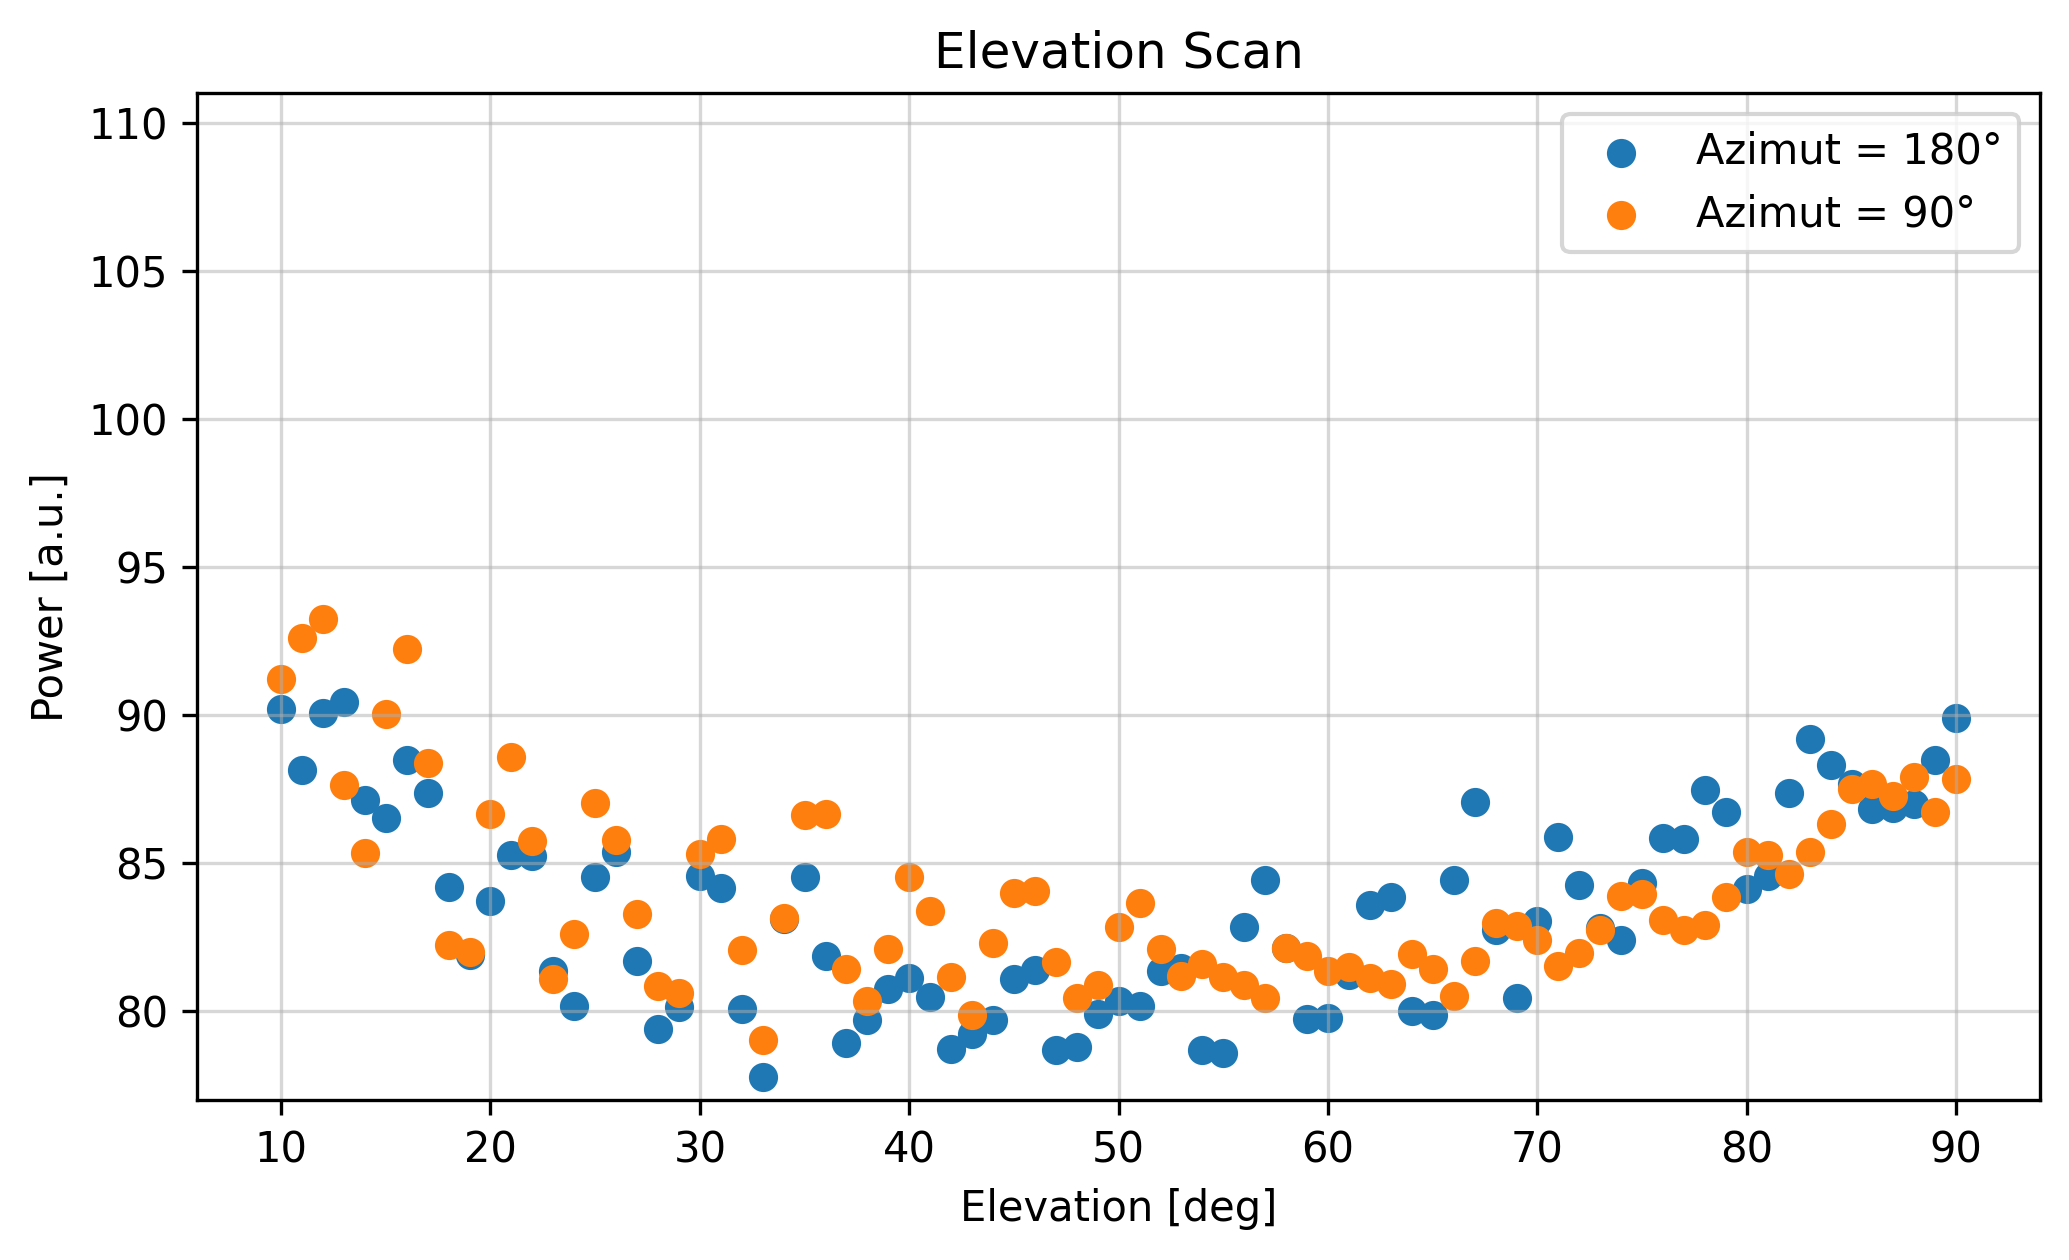
\includegraphics[width=\linewidth]{assets/elev_scan_night.png}
    \caption{Elevation Scan \texttt{01.10.2025 22:35 MESZ}}
\end{subfigure}
\begin{subfigure}[t]{0.45\textwidth}
    \centering
    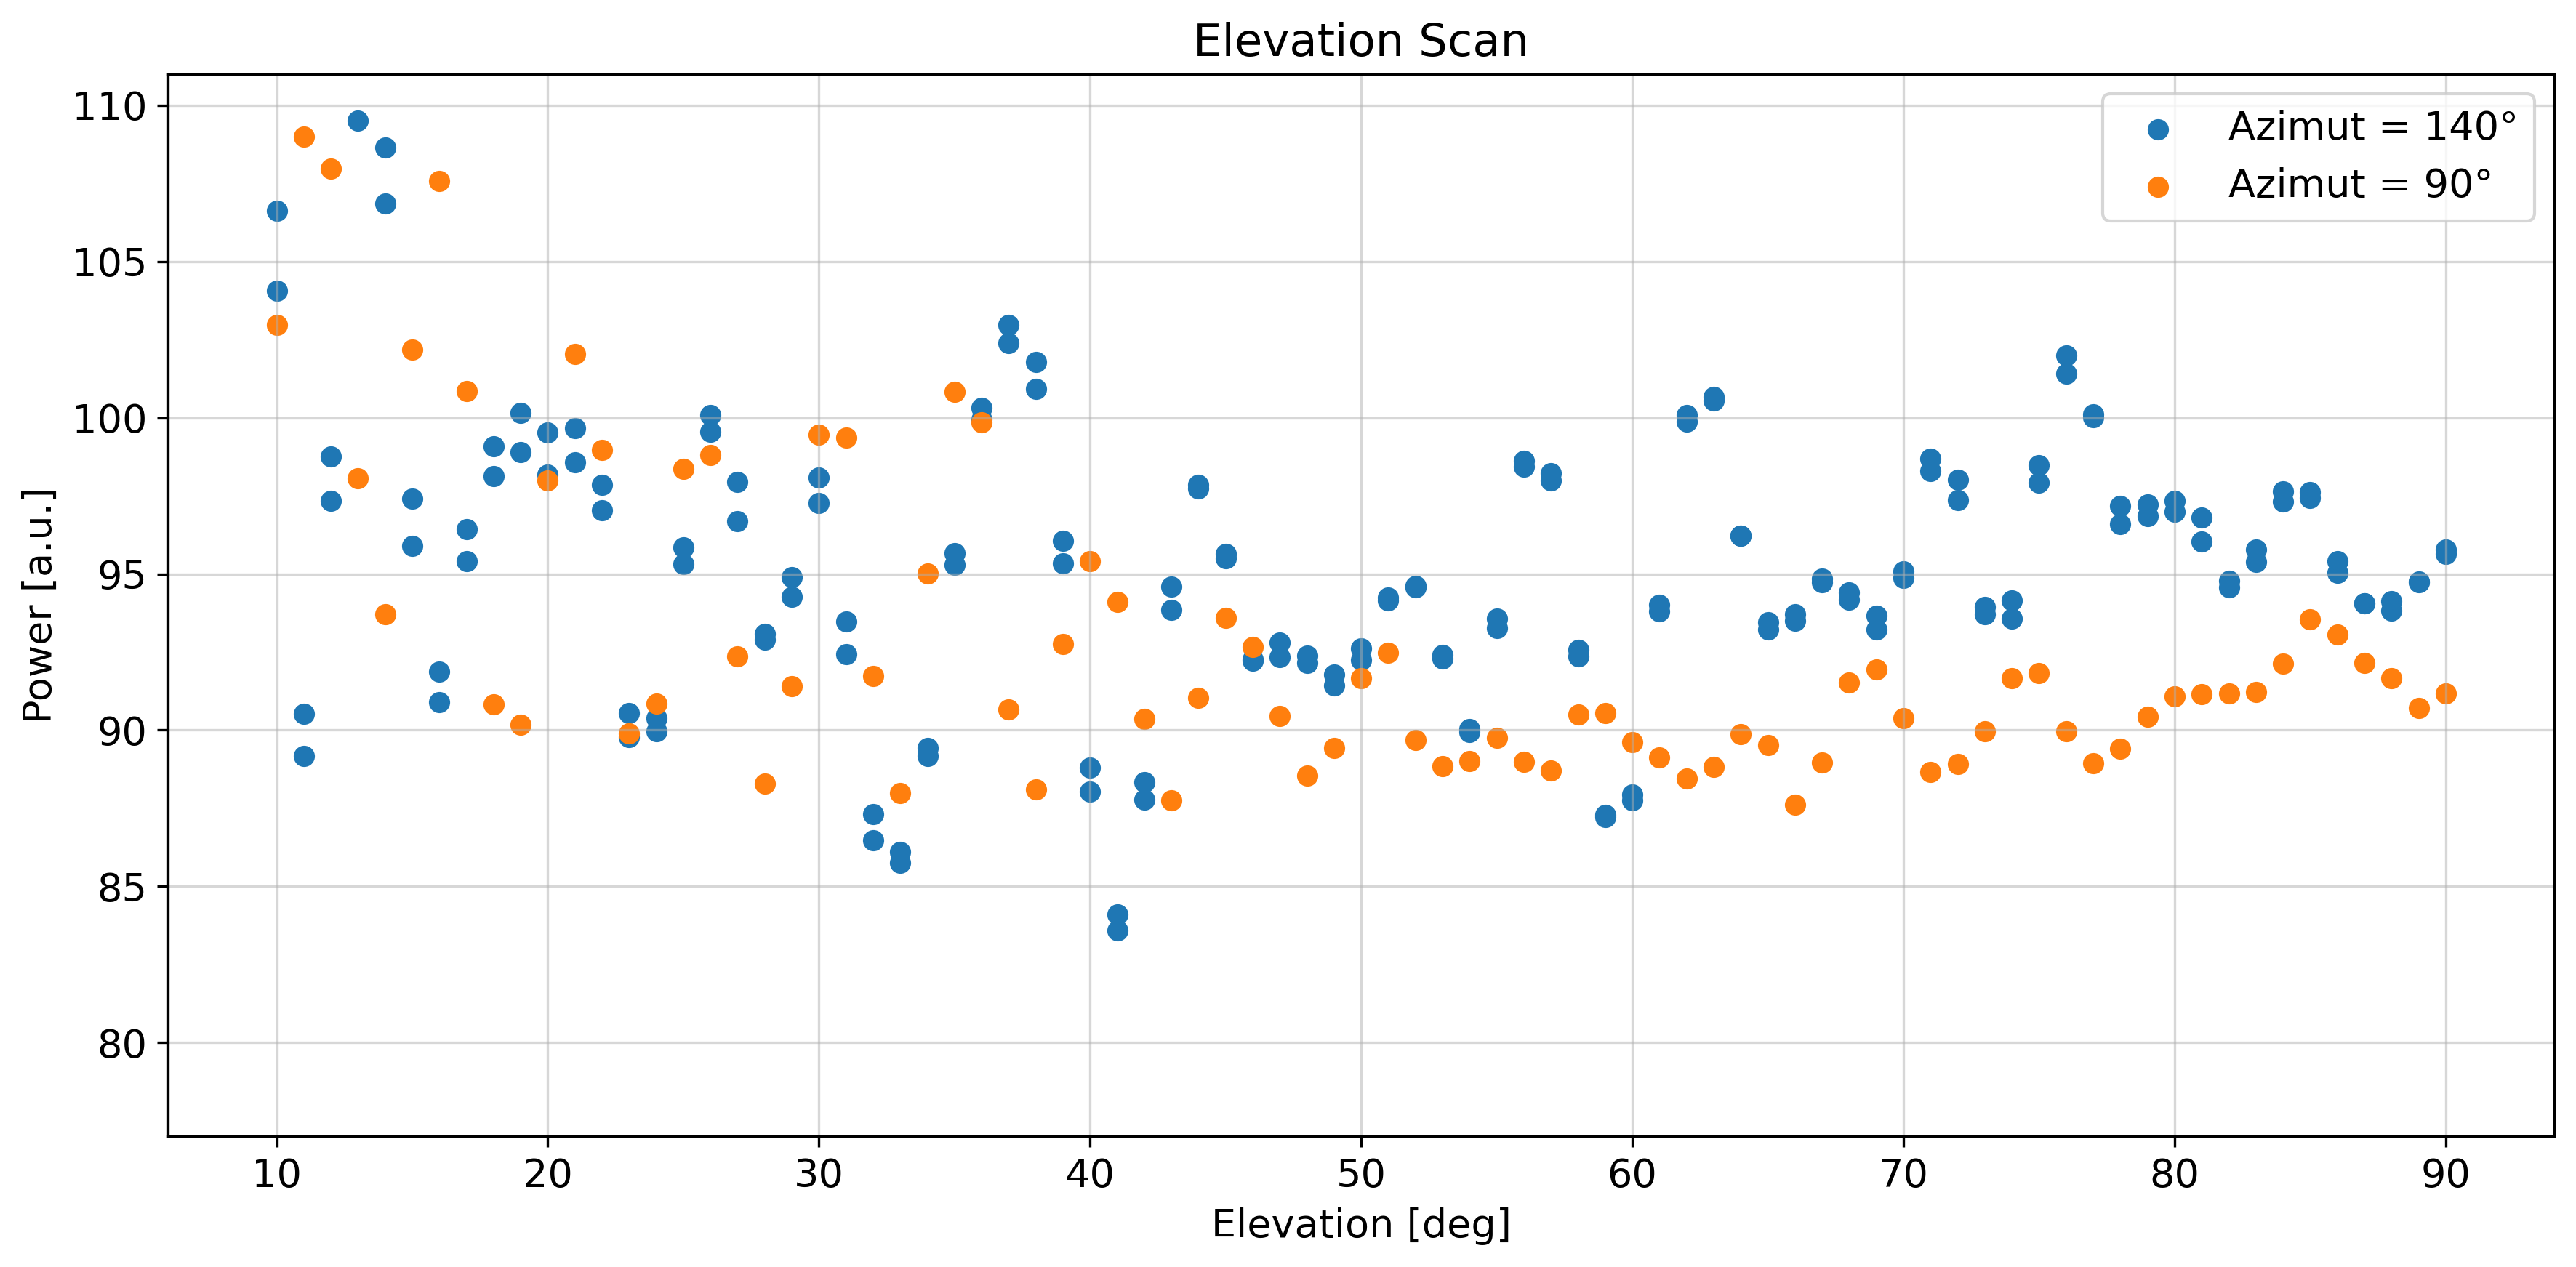
\includegraphics[width=\linewidth]{assets/elev_scan_day.png}
    \caption{Elevation Scan \texttt{02.10.2025 13:00 MESZ}}
\end{subfigure}
\caption{Elevation Scans at diffrent times of the day}
\label{fig:elev_scan}
\end{figure}

We notice that, both during the day and at night, the signal is stronger for low elevations. During the night we notice that additionally the signal gets stronger as we approach the zenith.

To investaigate this further we looked at the celestial bodies that where near the zenith during that time. A screenshot of this, taken in Stellarium is shown in Figure \ref{fig:stellarium}. We notice, that the milky way is in the zenith during our time of measurement.

\begin{figure}[ht]
    \centering
    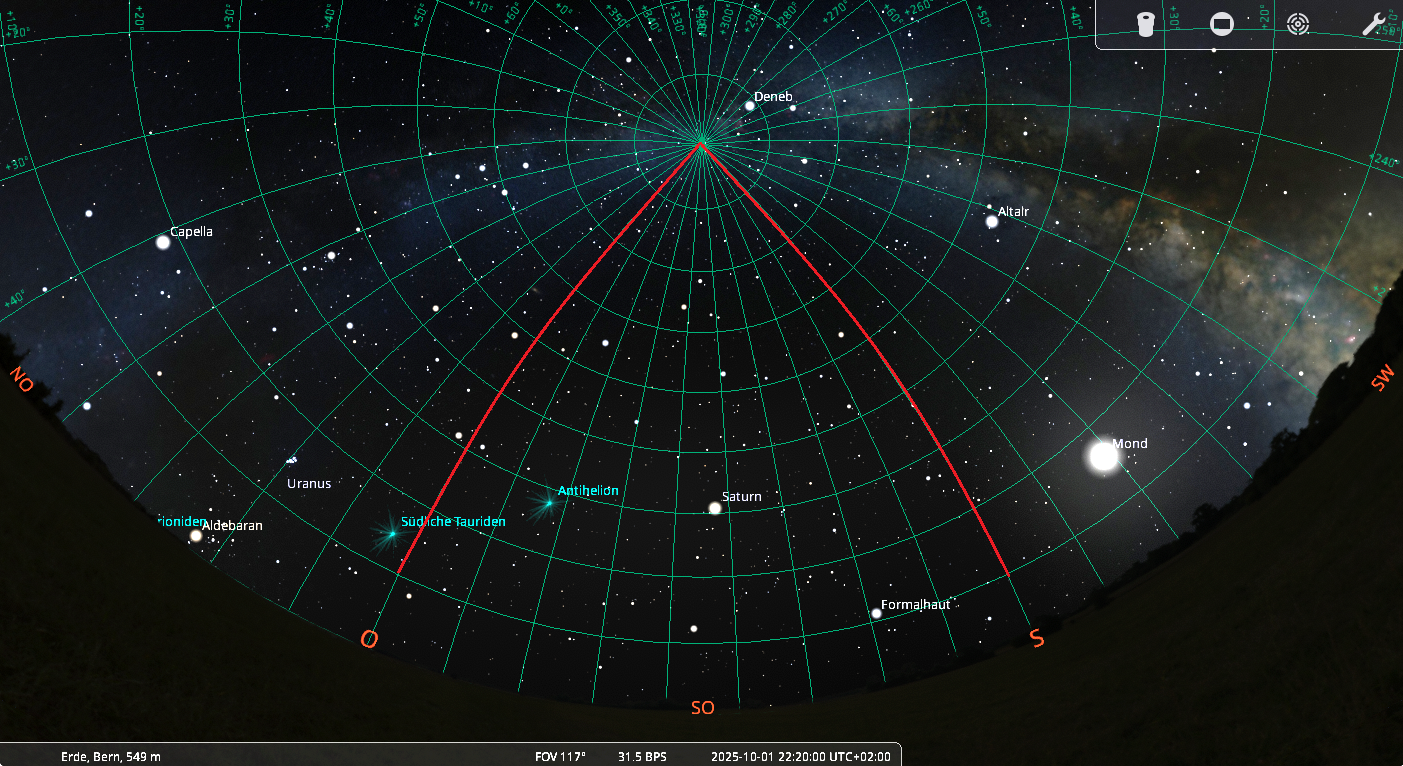
\includegraphics[width=0.6\linewidth]{assets/ElevationScan_Az90_Az180_251001_2220MESZ.png}
    \caption{View of the sky at \texttt{01.10.2025 22:20 MESZ}}
    \label{fig:stellarium}
\end{figure}

In Figure \ref{fig:elev_spectra} we plot the Spectral power density both at day and night for an elevation where near the minima shown in Figure \ref{fig:elev_scan}. We notice that during the day the spectra are a close match, and during the night we have a source with a frequency near the Carrier frequency, this would match with the \ce{H_I} we expect to be present in the milky-way.

Because of this we think that the increase in Power that is only observed during the night is caused by the scan path intercepting the milky-way near the zenith.
\begin{figure}[ht]
\centering
\begin{subfigure}[t]{0.45\textwidth}
    \centering
    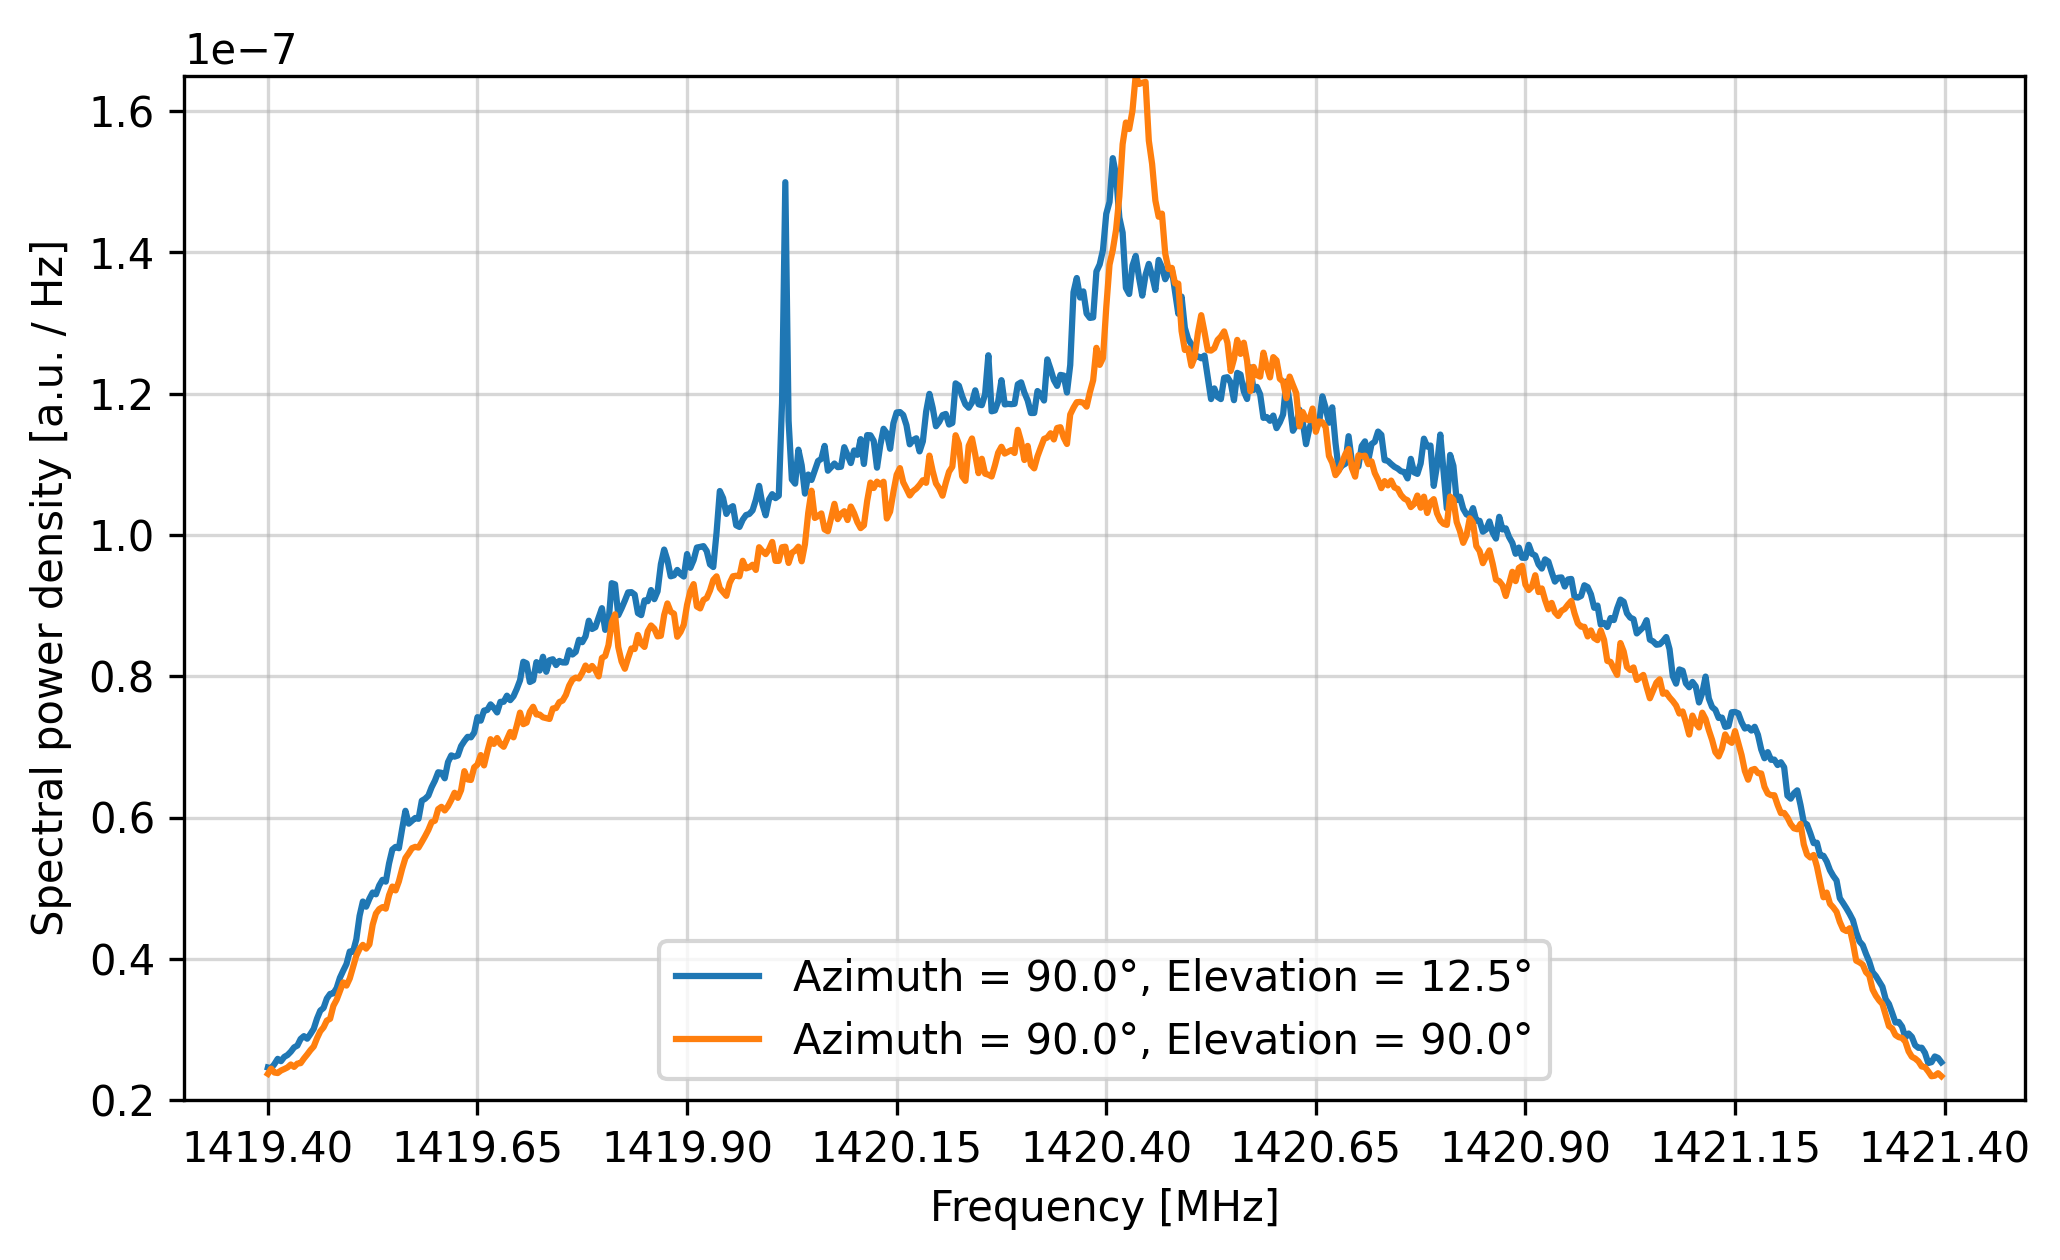
\includegraphics[width=\linewidth]{assets/elev_spectrum_night.png}
    \caption{Spectra for two different elevations\\ \texttt{01.10.2025 22:35 MESZ}}
\end{subfigure}
\begin{subfigure}[t]{0.45\textwidth}
    \centering
    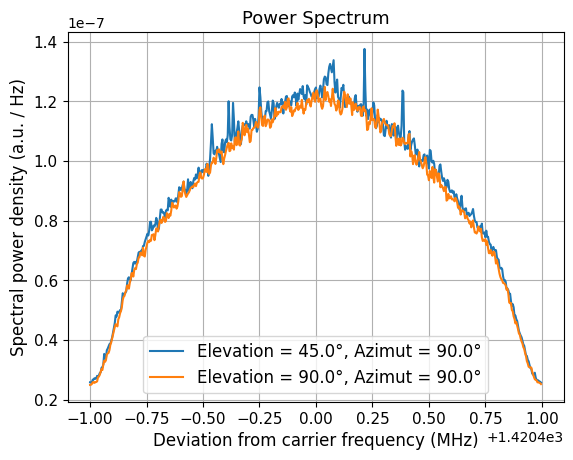
\includegraphics[width=\linewidth]{assets/elev_spectrum_day.png}
    \caption{Spectra for two different elevations\\ \texttt{02.10.2025 13:00 MESZ}}
\end{subfigure}
\caption{Spectra at diffrent Elevations and diffrent times of the day}
\label{fig:elev_spectra}
\end{figure}


TODO: correct Az/Elv. Do same y-range *******************************************